 \begin{sloppypar}
\chapter{Sviluppi Futuri}
\section{Introduzione}
\fontsize{12}{19}\selectfont{
Nel corso dell’ultimo decennio sono stati condotti numerosi studi sull’applicazione della robotica nel campo della disabilità. 
La terapia assistita da robot è un campo di ricerca ed applicazione promettente \cite{Numero12}, un’altra delle sfide che tecnologia e clinica affrontano insieme allo scopo di supportare i pazienti. Una parte rilevante delle attuali ricerche si è focalizzata sull’utilità delle tecnologie robotiche nello stimolare le abilità deficitarie nei Disturbi dello Spettro Autistico, dando conferma di come i robot umanoidi possano fornire un valido aiuto nel creare una comunicazione con il paziente, favorendone l’attenzione e generando nuovi comportamenti sociali.\newline
Dagli studi che si sono succeduti negli anni, è emerso che i robot umanoidi, senza mai  sostituirsi all’essere umano, migliorano le competenze sociali dei pazienti, per i quali l’interazione con le altre persone è un elemento che disorienta, anche a causa della variegata espressività del volto umano; interagendo con una persona, i pazienti affetti da DSA vengono a contatto con numerosi segnali sociali (le espressioni facciali, i gesti, la tonalità della voce) per loro difficili da interpretare.\newline
Il robot diventa quindi una sorta di intermediario, affidabile e prevedibile, uno strumento conoscitivo per apprendere maggiori informazioni sul funzionamento della mente dei pazienti e di supporto per un percorso diagnostico e terapeutico completo.
\vspace{1.5cm}
\begin{figure}[H]
\centering
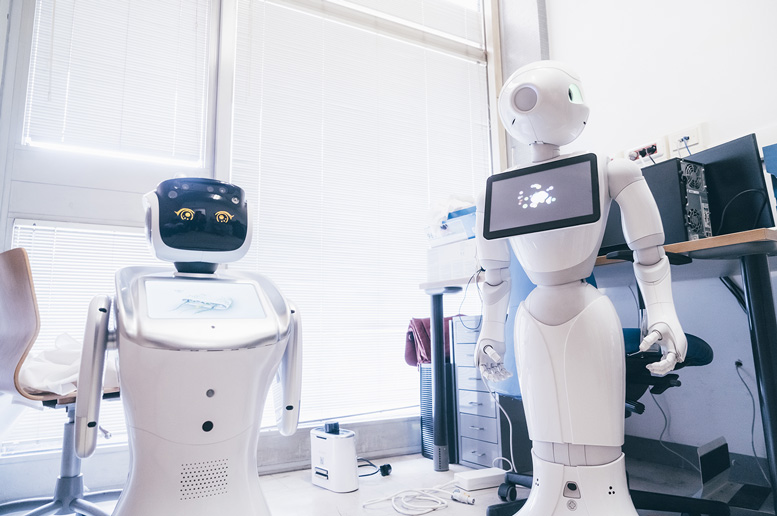
\includegraphics[width=0.8\textwidth]{immagini/pepper_finale.jpg}
\caption{Robot assistenziali utilizzati nel reparto di pediatria dell'ospedale di Padova}
\end{figure}
\vspace{1cm}
\newpage
Nel prossimo futuro, si prevede che l’Intelligenza Artificiale parteciperà in modo progressivo ai processi decisionali in ambito sanitario e i professionisti del settore  utilizzeranno sempre più dispositivi di intelligenza artificiale e apprendimento automatico per migliorare la precisione nella diagnosi e identificare i regimi terapeutici.\newline
Tuttavia, pur offrendo numerose possibilità anche molto promettenti, l’adozione dei robot di assistenza rimane ancora inferiore al previsto, per un gap tra tecnologia e assistenza sanitaria. Gap che non deriva esclusivamente dalle attuali strategie per l’implementazione dei robot, ma è piuttosto un gap informativo nelle sezioni trasversali della progettazione tecnologica, della sanità e della società.\newline
E’ necessaria una diffusione delle conoscenze che favorisca l’interazione e la condivisione delle informazioni tra tutte le parti interessate coinvolte  nella gestione dei robot per la diagnosi e cura dei DSA. La progettazione e l'implementazione di un robot richiedono competenze multidisciplinari provenienti da settori quali l'ingegneria, l'informatica, la psicologia e la riabilitazione clinica e la collaborazione tra i professionisti delle diverse discipline può portare ad un numero maggiore di contributi in questa area di ricerca con conseguenti ricadute positive sui pazienti.
\newline
Rimangono importanti i punti a favore della terapia assistita da robot. Essendo trattamenti informatizzati, è possibile tracciare e monitorare i progressi e gli step del trattamento, senza la necessità di affidarsi alle tecniche di osservazione tradizionali, personalizzando e adattando i percorsi alle specifiche esigenze del singolo paziente.\newline
I disturbi dello spettro autistico si caratterizzano per la grande variabilità che c’è tra un soggetto e l’altro e la possibilità di avere strumenti condivisi ma personalizzabili è sicuramente di grande vantaggio per i clinici.
Una delle sfide più ardue è quella di rendere le soluzioni tecnologiche offerte dalla robotica assistiva usabili ed accettabili per i soggetti che dovrebbero trarne beneficio. Questo passaggio è tutt’altro che scontato. In questo senso, un approccio che nasce nel mondo dell’architettura e del design, ma che tende progressivamente ad estendersi alla progettazione di soluzioni tecnologiche ovvero di servizi integrati con soluzioni tecnologiche, è il cosiddetto \textit{Human Centered Approach}. Il punto cardine di questo modello, come evidenziato dal nome, consiste nel mettere al centro della progettazione la persona e i suoi bisogni, per far sì che i desideri e le aspettative da questa espressi siano la linea guida per lo sviluppo del prodotto o servizio. Infine, esso mira ad includere la prospettiva di tutti coloro che possono avere un interesse nella realizzazione e ad assumere quindi non solo il punto di vista dell’utente finale ma anche quello di eventuali operatori, manutentori, specialisti, etc.
}
\newpage
\section{Funzionalità future dell' applicazione}
\fontsize{12}{19}\selectfont{Attraverso l’impiego di tecnologie avanzate e l’applicazione di principi psicologici specifici, definiti anche grazie alla collaborazione con professionisti del settore, è stato possibile realizzare uno strumento accessibile, intuitivo e personalizzabile.\newline
Al momento sono in fase di studio e realizzazione nuove possibili funzionalità dell’applicazione, in particolare una dashboard e un database dedicato, come di seguito descritte:
\vspace{0.5cm}
\begin{enumerate}
    \item \textbf{Dashboard}: interfaccia \textit{user-friendly} di supporto ai clinici per avere accesso immediato alla raccolta di tutti i test da somministrare ai pazienti e per monitorarne i progressi durante la terapia nel corso del tempo. 
    \vspace{0.5cm}
    \item \textbf{Database dedicato}: organizzazione strutturata delle informazioni raccolte da Pepper, per consentirne il salvataggio, la visualizzazione e un facile reperimento da parte degli utenti.\newline
    Il database da utilizzare memorizzerà le seguenti informazioni:
    \begin{itemize}
     \vspace{0.5cm}
    \item Parametri facciali univoci associati ad  un dato paziente e restituiti dal modulo di riconoscimento facciale del robot.
     \vspace{0.5cm}
    \item Informazioni anagrafiche e sanitarie, contenenti la storia clinica di ogni paziente.
     \vspace{0.5cm}
        \item Registrazione video delle sedute di somministrazione dei test, identificate dal codice univoco di ogni paziente e dalla data di acquisizione.
         \vspace{0.5cm}
        \item Registrazione audio delle sedute di somministrazione dei test, identificate dal codice univoco di ogni paziente e dalla data di acquisizione.
    \end{itemize}
\end{enumerate}
}
 \end{sloppypar}
\afterpage{\blankpage}